\documentclass[10 pt, a4paper]{beamer}
\usetheme{metropolis}          
\usecolortheme{metropolis} 
\usepackage[utf8]{inputenc}
\usepackage{amsmath,amsfonts,amssymb}
\usepackage{dsfont}
\usepackage{graphicx}
\usepackage{caption}
\usepackage[french]{babel}
\usefonttheme[onlymath]{serif}


\title{Étude du problème MP-LWE}
\date{31 Août 2023}
\author{Sacha Ben-Arous}
\institute{ENS Paris-Saclay}
\begin{document}
  \maketitle
  
\begin{frame}{Plan}
\tableofcontents
\end{frame}  

%def Z_p
%écrire A
%donner les noms PLWE MPLWE et parler du produit
%Pas parler de pq avoir le rang plein c'est pratique

\section{Introduction aux réseaux}

\subsection{Définition}


\begin{frame}{Définition}
\onslide<1->{Un \textbf{réseau euclidien} de $\mathbb{R}^m$ est l'ensemble des combinaisons à coefficients entiers de vecteurs linéairements indépendants $b_1, \dots, b_n$, que l'on note :
\[\mathcal{L}(b_1,\dots,b_n) := \left\{ \sum_{i=1}^n x_ib_i, x_i \in \mathbb{Z} \right\} \]}

\onslide<2->{Le réseau est alors de \textit{dimension} $n$, et la famille des $(b_i)_{1\leq i \leq n}$ est appelée \textbf{base} de ce réseau.}\\
\onslide<3->{~ \\ En notant $B:=[b_1,\dots,b_n]$, on considérera de manière équivalente : \[\mathcal{L}(B) := \left\{ Bx, x \in \mathbb{Z}^n \right\} \]}
\end{frame}



\begin{frame}{Exemples}
\begin{center}
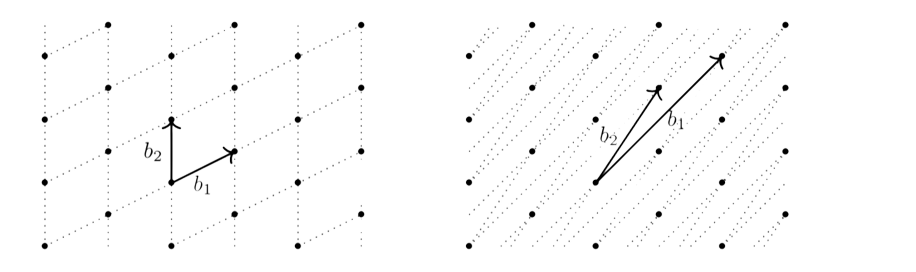
\includegraphics[scale=0.38]{lattice.png}
\captionof{figure}{Exemple de réseau [Kat23]}
\end{center}
\end{frame}


\subsection{Learning With Errors}
\begin{frame}{Learning With Errors}
\textbf{Learning With Errors Problem :} \\ ~ \\
\onslide<1->{On fixe des entiers $n$ et $t$, un nombre premier $q$ et une distribution de bruit $\mathcal{N}(\sigma)$. On tire un secret $s\hookleftarrow \mathcal{U}(\mathbb{Z}_q^n)$.  \\ ~ \\}

\onslide<2->{Le problème est le suivant : à partir de $t$ échantillons \[(a_i,b_i):=(a_i,\left<a_i,s\right> +e_i \text{ mod } q)\] où $a_i\hookleftarrow \mathcal{U}(\mathbb{Z}_p^n)$ et $e_i\hookleftarrow \mathcal{N}(\sigma)$, on souhaite retrouver le secret $s$. \\ ~ \\}
\onslide<3->{\underline{Rq} : Sans bruit, le problème est facile à résoudre.}
\end{frame}

\begin{frame}{Lien avec les réseaux}
Cela revient à chercher le point le plus proche de $A\cdot s + e$ dans le réseau engendré par \onslide<1>{A} \\ ~ \\ \onslide<2>{$A' := 
 \left[\begin{array}{c|ccc}
&q&\cdots & 0\\
A & \vdots &\ddots & \vdots\\
 & 0 & \cdots &q\\
\end{array}\right]
\in \mathbb{Z}^{t\times (n+t)}$
car on travaillait modulo $q$}
\end{frame}


\begin{frame}{Difficulté de LWE}
\begin{itemize}
\item<1->[•]La difficulté est relié au facteur $\gamma = \frac{\lambda_1}{\|e\|}$ \\ ~ \\
\item<2->[•] Plus $\gamma$ est petit, plus le problème est dur \\ ~ \\
\item<3->[•] Si $\gamma = poly(n)$, ce problème est conjecturé exponentiellement dur à résoudre, même sur un ordinateur quantique
\begin{center}
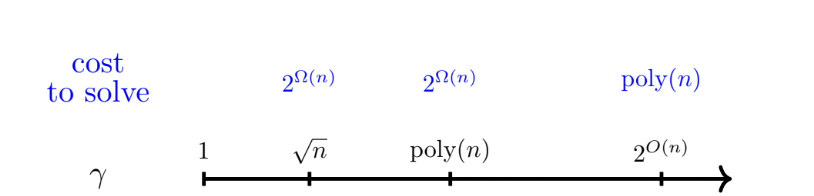
\includegraphics[scale=0.30]{gamma_hard.png}
\captionof{figure}{Lien difficulté/gamma [Kat23]}
\end{center}
\end{itemize}
\end{frame}

\subsection{Variantes structurées}
\begin{frame}{Variantes structurées}
\onslide<1->{\textbf{Problème }: LWE tel quel est peu efficace à cause des grandes matrices aléatoires. \\ ~ \\}
\onslide<2->{\textbf{Solution } : Rajouter de la structure : polynômes (Stehlé \textit{et al.} [SSTX09])}
\end{frame}


\begin{frame}{Illustration}
Concrètement, cela consiste à représenter matriciellement le produit de polynômes, et donc à mettre des blocs structurés dans $A$
\begin{center}
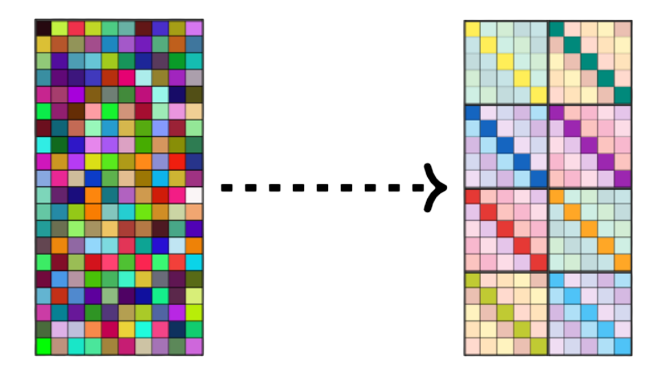
\includegraphics[scale=0.30]{plwe_struct.png}
\captionof{figure}{Représentation de la structure d'un réseau [Kat23]}
\end{center}
\end{frame}


\begin{frame}{Variantes structurées}
\onslide<1->{Défaut : nouveau paramètre $f \in \mathbb{Z}^m_q[X]$ qui régit la complexité. \\ ~ \\}
\onslide<1->{\underline{Ex }: $x^n+1$ et $x^n -1$ \\ ~ \\}
\onslide<2->{Roşca \textit{et al.} [RSSS17] introduisent une nouvelle variante structurée, et y réduisent des classes exponentiellement grandes de problèmes P-LWE.}
\end{frame}


\section{Étude de la réduction}


\begin{frame}{Objectif}
\begin{itemize}
\item<1->[•] Comprendre le fonctionnement de la réduction, et son impact sur les paramètres de difficulté.  \\ ~ \\
\item<2->[•] Établir des propriétés sur le nouveau réseau d'arrivée 
\end{itemize}
\end{frame}

\subsection{Heuristique gaussienne}
\begin{frame}{Représentation matricielle de la réduction}
\onslide<1->{On défini $\text{Rot}_f(a)$ pour qu'elle vérifie $\text{Rot}_f(a) \cdot b = (a\times b \mod f)$ \\ ~ \\}
\onslide<2->{\underline{Ex}: Si $f=x^4+1$ et $\displaystyle a=\sum_{0\leq i < 4} a_ix^i$, alors :
$$
\text{Rot}_f(a) = \begin{pmatrix}
a_0 & a_1 & a_2 & a_3 \\
-a_3 & a_0 & a_1 & a_2 \\
-a_2 & -a_3 & a_0 & a_1 \\
-a_1 & -a_2 & -a_3 & a_0 \\
\end{pmatrix} 
$$
}

\end{frame}


\begin{frame}{Représentation matricielle de la réduction}
\onslide<1->{De même pour $\text{Toep}_d(a)$, choisie pour avoir $\text{Toep}_d(a) \cdot b = (a\odot_d b)$ \\ ~ \\}
\onslide<2->{\underline{Ex}: Si  $d=4$ et $\displaystyle a=\sum_{0\leq i < 4} a_ix^i$, alors :
$$
\text{Toep}(a) = \begin{pmatrix}
a_0 & a_1 & a_2 & a_3 &0&0&0\\
0&a_0 & a_1 & a_2 & a_3&0&0 \\
0&0&a_0 & a_1 & a_2 & a_3&0 \\
0&0&0&a_0 & a_1 & a_2 & a_3 \\
\end{pmatrix} 
$$
}

\end{frame}


\begin{frame}{Représentation matricielle de la réduction}
La réduction va donc de 
$
A_1= 
\left[ \begin{array}{c}
\text{Rot}_f(a_1) \\
\vdots  \\
\text{Rot}_f(a_t) \\
\end{array} \right]
$
vers 
$
A_2= 
\left[ \begin{array}{c}
\text{Toep}_d(a_1) \\
\vdots  \\
\text{Toep}_d(a_t) \\
\end{array} \right]
$

\end{frame}

\begin{frame}{Heuristique gausienne}
\onslide<1->{Volume d'un réseau $\mathcal{L}(B)$  $ := \sqrt{\det{(B^\top B)}}$. \\ ~ \\
\underline{Rq }: ne dépend pas de $B$\\ ~ \\ }
\onslide<2->{\textbf{Heuristique gaussienne : }\[ |\{\text{points du réseau de norme} \leq R \}| \simeq \frac{V_n(R)}{\text{vol}(L)} = \frac{R^n V_n(1)}{\text{vol}(L)}\]
En particulier $\lambda_1 \simeq \sqrt{n} \cdot \text{vol}(L)^\frac{1}{n}$}
\end{frame}

\subsection{Volume et erreur}
\begin{frame}{Volumes}
\onslide<1->{\textbf{Théorème : } Avec probabilité $\geq 1 - \frac{1}{q^{mt}}$ on a $\text{vol}(\mathcal{L}_1) = q^{m(t-1)}$ \\ ~ \\}
\onslide<2->{\textbf{Théorème : }Avec une probabilité $\geq 1 - (\frac{n+d-1}{q})^{\lfloor t/\lceil\frac{n+d-1}{d}\rceil\rfloor}$, on a que $\text{vol}(\mathcal{L}_2)=q^{td-(n+d-1)}$ \\ ~ \\}
\onslide<3->{À retenir : $\frac{\text{vol}(\mathcal{L}_1)^\frac{1}{tm}}{\text{vol}(\mathcal{L}_2)^\frac{1}{td}} = q^\frac{n}{td}$, et $td \simeq n$ donc le volume change peu}
\end{frame}


\begin{frame}{Idée de preuve}
\begin{itemize}
\item<1->[•] Il suffit d'avoir que $A_1$ et $A_2$ sont de rang plein\\ ~ \\
\item<2->[•] Pour $A_1$ : utiliser $\text{Rot}_f(a)^{-1}=\text{Rot}_f(a^{-1})$\\ ~ \\
\item<3->[•] Pour $A_2$ : plus dur car bloc pas carrés, il faut les rassembler. Ma preuve n'utilise pas la structure Toeplitz, et la borne est non optimale.
\end{itemize}
\end{frame}


\begin{frame}{Résultats expérimentaux}
$n=22$, $d=11, t=3$, et $q=n^\beta\log{n}$ où on fait varier $\beta$. En pratique $n$ est beaucoup plus grand, et dans le schéma $\beta=2.5$. En faisant $10^6$ tests, on obtient les résultats suivants : \\

\begin{center}
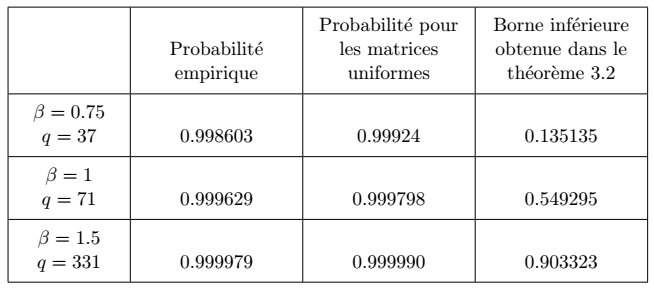
\includegraphics[scale=0.40]{tab_exp.png}
\end{center}
\end{frame}

\begin{frame}{Erreurs}
\begin{itemize}
\item[•] $\mathbb{E}(\|e_1\|^2) = tm(\alpha q)^2 $\\ ~ \\
\item[•] $\mathbb{E}(\|e_2\|^2) = td(\alpha d S q)^2$ \\ ~ \\
\end{itemize}

car $\sigma_2 = (\alpha d S)\sigma_1$. Voir rapport pour détails.
\end{frame}

\begin{frame}{Heuristique gaussienne}
\onslide<1->{\textbf{Théorème (Minkowski) :} $\lambda_1 \leq \sqrt{n}\cdot\text{vol}(\mathcal{L})^\frac{1}{n}$  \\ ~ \\ }
\onslide<2->{\textbf{Théorème : } Si $d=\frac{n}{2}$ et $t\geq 4$ alors, avec probabilité $\displaystyle \geq 1-\frac{1}{2^{td-1}q^{t-3}}$, on a : \[\lambda_1^\infty(\mathcal{L}_2) \geq \frac{1}{2q} \text{vol}(\mathcal{L}_2)^{\frac{1}{dt}}\]}

\onslide<3->{\underline{Rq }: Le résultat est en norme infinie, et est trop faible par rapport à ce qui attendu.}

\end{frame}


\subsection{Schéma de chiffrement}
\begin{frame}{Schéma de chiffrement}
\onslide<1->{\textbf{Théorème [RSS17] : }
Si $\alpha \leq \frac{1}{16\sqrt{tk\lambda}}$ et  $16t(k+1)\leq q$, alors pour tout $\mu \in \{0,1\}^{<d}[X]$, avec probabilité $\geq 1 - 2^{-\Omega(\lambda)}$ sur $\texttt{(sk,pk)}\hookleftarrow\texttt{KeyGen} $, on a $\texttt{Decrypt(sk,Encrypt(pk,mu)) = mu}$ \\ ~ \\

Preuve incorrecte, j'en donne une nouvelle version, avec des hypothèses renforcées.\\ ~ \\}

\onslide<2->{\textbf{Théorème :}
Si $\alpha \leq \frac{1}{16(k+1)t\sqrt{\lambda}}$ et  $8td(k+1)\leq qd\leq e^\lambda$, alors pour tout $\mu \in \{0,1\}^{<d}[X]$, avec probabilité $\geq 1 - 2^{-\Omega(\lambda)}$ sur $\texttt{(sk,pk)}\hookleftarrow\texttt{KeyGen} $, on a $\texttt{Decrypt(sk,Encrypt(pk,mu)) = mu}$\\ ~ \\}


\onslide<3->{\underline{Rq} : La modification est essentiellement au niveau de $\alpha$, que l'on a diminué. Cela a pour effet de réduire la variance de l'erreur gaussienne appliquée sur le message, ce qui le rend plus simple à déchiffrer, et facilite donc la preuve.}
\end{frame}


\begin{frame}{Conclusion}
\begin{itemize}
\item[•] MP-LWE gagne sur le plan algébrique tout en conservant la difficulté algorithmique\\ ~ \\
\item[•] Résultat sur l'heuristique gaussienne à améliorer\\ ~ \\
\item[•] Étudier l'influence de la structure sur le rang des réseaux
\end{itemize}
\end{frame}


\begin{frame}{Références}
[Kat23] \ Katharina Boudgoust, ``Hardness Assumptions in Lattice-Based Cryptography" \\ ~ \\
RSSS17] \ Miruna Roşca , Amin Sakzad, Damien Stehlé et Ron Steinfeld ``Middle-Product Learning With Errors"\\ ~ \\
SSTX09] \ Damien Stehlé, Ron Steinfeld, Keisuke Tanaka et Keita Xagawa “Efficient public key encryption based on ideal lattices"
\end{frame}
\end{document}













































